%-----------------------------------------------------------------------------------------------------------------------------------------------%
%	The MIT License (MIT)
%
%	Copyright (c) 2021 Jitin Nair
%
%	Permission is hereby granted, free of charge, to any person obtaining a copy
%	of this software and associated documentation files (the "Software"), to deal
%	in the Software without restriction, including without limitation the rights
%	to use, copy, modify, merge, publish, distribute, sublicense, and/or sell
%	copies of the Software, and to permit persons to whom the Software is
%	furnished to do so, subject to the following conditions:
%	
%	THE SOFTWARE IS PROVIDED "AS IS", WITHOUT WARRANTY OF ANY KIND, EXPRESS OR
%	IMPLIED, INCLUDING BUT NOT LIMITED TO THE WARRANTIES OF MERCHANTABILITY,
%	FITNESS FOR A PARTICULAR PURPOSE AND NONINFRINGEMENT. IN NO EVENT SHALL THE
%	AUTHORS OR COPYRIGHT HOLDERS BE LIABLE FOR ANY CLAIM, DAMAGES OR OTHER
%	LIABILITY, WHETHER IN AN ACTION OF CONTRACT, TORT OR OTHERWISE, ARISING FROM,
%	OUT OF OR IN CONNECTION WITH THE SOFTWARE OR THE USE OR OTHER DEALINGS IN
%	THE SOFTWARE.
%	
%
%-----------------------------------------------------------------------------------------------------------------------------------------------%

%----------------------------------------------------------------------------------------
%	DOCUMENT DEFINITION
%----------------------------------------------------------------------------------------

% article class because we want to fully customize the page and not use a cv template

%%%% DEBUG COMMAND
%%%%\listfiles


%----------------------------------------------------------------------------------------
%	FONT
%----------------------------------------------------------------------------------------

% % fontspec allows you to use TTF/OTF fonts directly
% \usepackage{fontspec}
% \defaultfontfeatures{Ligatures=TeX}

% % modified for ShareLaTeX use
% \setmainfont[
% SmallCapsFont = Fontin-SmallCaps.otf,
% BoldFont = Fontin-Bold.otf,
% ItalicFont = Fontin-Italic.otf
% ]
% {Fontin.otf}

%----------------------------------------------------------------------------------------
%	PACKAGES
%----------------------------------------------------------------------------------------
\usepackage{url}
\usepackage{parskip} 	

%other packages for formatting
\RequirePackage{color}
\RequirePackage{graphicx}
\usepackage[usenames,dvipsnames]{xcolor}
\usepackage[scale=0.9]{geometry}

%tabularx environment
\usepackage{tabularx}

%for lists within experience section
\usepackage{enumitem}

% centered version of 'X' col. type
\newcolumntype{C}{>{\centering\arraybackslash}X} 

%to prevent spillover of tabular into next pages
\usepackage{supertabular}
\usepackage{tabularx}
\newlength{\fullcollw}
\setlength{\fullcollw}{0.47\textwidth}

%custom \section
\usepackage{titlesec}				
\usepackage{multicol}
\usepackage{multirow}

%CV Sections inspired by: 
%http://stefano.italians.nl/archives/26
\titleformat{\section}{\Large\scshape\raggedright}{}{0em}{}[\titlerule]
\titlespacing{\section}{0pt}{10pt}{10pt}

%\titleformat{\subsection}{}{}{}{}[\titlerule]
%\titlespacing{\subsection}{0pt}{10pt}{10pt}


%for publications
%\usepackage[style=authoryear,sorting=ynt, maxbibnames=2]{biblatex}
%\usepackage[style=authoryear,sorting=ydnt,maxbibnames=100]{biblatex}

\usepackage[%backend=biber,
        style=numeric,
        %        sorting=ydnt,
        sorting=ymdDnt,
        maxbibnames=100,
        defernumbers=true,
%        dateabbrev=false, % abbrev month display
        alldates=long]{biblatex}

% SORT BY YEAR, MONTH, DAY (decreasing)
\DeclareSortingTemplate{ymdDnt}{
  \sort{
    \field{presort}
  }
  \sort[final]{
    \field{sortkey}
  }
  \sort[direction=descending]{
    \field{sortyear}
    \field{year}
    \literal{9999}
  }
  \sort[direction=descending]{
    \field[padside=left,padwidth=2,padchar=0]{month}
    \literal{99}
  }
  \sort[direction=descending]{
    \field[padside=left,padwidth=2,padchar=0]{day}
    \literal{99}
  }
  \sort{
    \field{sortname}
    \field{author}
    \field{sorttitle}
    \field{title}
  }
  \sort{
    \field{sorttitle}
  }
  \sort[direction=descending]{
    \field[padside=left,padwidth=4,padchar=0]{volume}
    \literal{9999}
  }
}








\defbibheading{subbibliography}[\refname]{\subsection{#1}}
\setcounter{secnumdepth}{0}



%% \usepackage[
%%   style=publist,
%%   maxnames=11,
%%   plnumbering=local,
%%   marginyear=true,
%% ]{biblatex}



%Setup hyperref package, and colours for links
\usepackage[unicode, draft=false,pdfauthor={David Doukhan (INA)},pdftitle={CV David Doukhan},pdfkeywords={machine learning, speech analysis, gender studies, computer vision}]{hyperref}
\definecolor{linkcolour}{rgb}{0,0.2,0.6}
\hypersetup{colorlinks,breaklinks,urlcolor=linkcolour,linkcolor=linkcolour}

% replace full url with hyperlink and symbol
\DeclareFieldFormat{url}{\mkbibacro{URL}\addcolon\space\href{#1}{\faExternalLink*}}
\newcommand{\myurl}[1]{URL:~\href{#1}{\faExternalLink*}}


\addbibresource{david_doukhan_ina.bib}
\addbibresource{david_doukhan_older.bib}
\addbibresource{david_doukhan_itw.bib}
\addbibresource{david_doukhan_unpublished.bib}
\setlength\bibitemsep{1em}

%for social icons
\usepackage{fontawesome5}

%debug page outer frames
%\usepackage{showframe}



%%% MYFILTER

\defbibcheck{nokeyword}{%
\iffieldundef{keywords}{}{\skipentry}}


\usepackage{tikz} 


%%% JOB COMMANDS

\newenvironment{jobshort}[2]
    {
    \begin{tabularx}{\linewidth}{@{}l X r@{}}
    \textbf{#1} & \hfill &  #2 \\[3.75pt]
    \end{tabularx}
    }
    {
    }

\newenvironment{joblong}[2]
    {
    \begin{tabularx}{\linewidth}{@{}l X r@{}}
    \textbf{#1} & \hfill &  #2 \\[3.75pt]
    \end{tabularx}
    \begin{minipage}[t]{\linewidth}
    \begin{itemize}[nosep,after=\strut, leftmargin=1em, itemsep=3pt,label=--]
    }
    {
    \end{itemize}
    \end{minipage}    
    }


%----------------------------------------------------------------------------------------
%	BEGIN DOCUMENT
%----------------------------------------------------------------------------------------
\begin{document}

% non-numbered pages
%\pagestyle{empty} 



%----------------------------------------------------------------------------------------
%	TITLE
%----------------------------------------------------------------------------------------

% \begin{tabularx}{\linewidth}{ @{}X X@{} }
% \huge{Your Name}\vspace{2pt} & \hfill \emoji{incoming-envelope} email@email.com \\
% \raisebox{-0.05\height}\faGithub\ username \ | \
% \raisebox{-0.00\height}\faLinkedin\ username \ | \ \raisebox{-0.05\height}\faGlobe \ mysite.com  & \hfill \emoji{calling} number
% \end{tabularx}

\begin{tabularx}{\linewidth}{@{} C @{}}
\Huge{David Doukhan, Ph.D.} \\[7.5pt]
\href{https://github.com/DavidDoukhan}{\raisebox{-0.05\height}\faGithub\ DavidDoukhan} \ $|$ \
\href{https://www.researchgate.net/profile/David-Doukhan}{\raisebox{-0.05\height}\faResearchgate\ David-Doukhan} \ $|$ \ 
\href{https://linkedin.com/in/david-doukhan}{\raisebox{-0.05\height}\faLinkedin\ david-doukhan}
%\href{https://mysite.com}{\raisebox{-0.05\height}\faGlobe \ mysite.com} \ $|$ \

\href{https://twitter.com/doukhan_david}{\raisebox{-0.05\height}\faTwitter \ doukhan\_david} \ $|$ \ 
\href{mailto:david.doukhan@gmail.com}{\raisebox{-0.05\height}\faEnvelope \ david.doukhan@gmail.com} \ $|$ \ 
\href{tel:+33678789781}{\raisebox{-0.05\height}\faMobile \ +33.6.78.78.97.81} \\
\end{tabularx}

\begin{tikzpicture}[remember picture, overlay]
  \node [anchor=north east, inner ysep=15pt, inner xsep=30pt]  at (current page.north east)
     {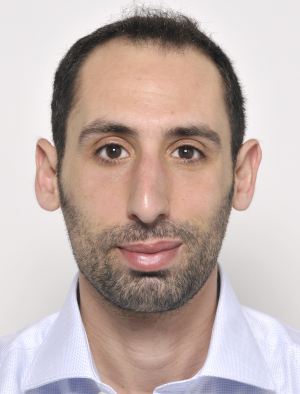
\includegraphics[height=3.2cm]{david_doukhan.jpg}};
\end{tikzpicture}

%\hfill
%\smash{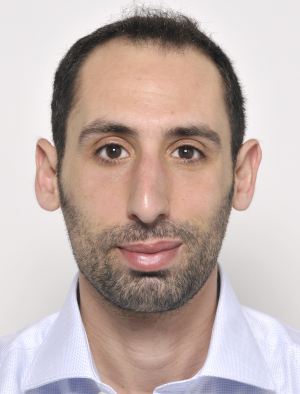
\includegraphics[width=2.5cm]{david_doukhan.jpg}}

%----------------------------------------------------------------------------------------
% EXPERIENCE SECTIONS
%----------------------------------------------------------------------------------------

%Interests/ Keywords/ Summary
\begin{en}
\section*{Summary}

I'm researcher at \href{https://www.ina.fr}{Institut National de l'Audiovisuel (INA)} in Paris metropolitan area (France).
This document presents some elements of my CV together with my detailed publication and research dissemination list (last update: \today).
More information to come!
%My research interest range from audio analysis and synthesis (audio segmentation, speaker diarization and recognition, paralinguistics, prosodic analysis 3D audio, speech synthesis), 
\end{en}

\begin{fr}
\section*{Résumé}

Je suis chercheur à l'\href{https://www.ina.fr}{Institut National de l'Audiovisuel (INA)} en région parisienne.
Mes travaux portent sur l'analyse automatique du signal audio (parole, musique, locuteur, prosodie, son 3D), l'apprentissage automatique, les humanités numériques (représentation de la diversité dans les médias), la linguistique de corpus et la gestion des collections audiovisuelles.
Ce document contient quelques éléments de mon CV, ainsi que la liste exhaustive de mes publications et travaux de dissémination scientifique (dernière mise à jour : \today).
\end{fr}



\tableofcontents

%% Experience
\begin{en}
\section{Work Experience}


\subsection{Research \& Engineering}

\begin{jobshort}{Audiovisual analysis Researcher at INA}{2016 - present}
Supervision of the speech analysis research group (2-3 interns, PhD students or engineers), involvement and coordination of national or European research projects, audiovisual analysis software implementation, gender representation studies, transfer of research results to production, governmental \& NGO reports
\end{jobshort}


\begin{jobshort}{Large-scale Music Information Retrieval Researcher at IRCAM}{2014-2015}
Distributed Machine-Learning algorithms implementation in Matlab, IRCAM’s classification framework refactorization, music genre and mood prediction
\end{jobshort}



\begin{jobshort}{Speaker analysis Researcher at LIMSI-CNRS}{2013-2014}
Speaker diarization and Voice Activity Detection for noisy archives (ethnographic recordings) in Python.
\end{jobshort}



\begin{jobshort}{Expressive Text-To-Speech at LIMSI-CNRS : Ph.D. Research}{2009-2013}
Annotated speech corpora production, inter-annotator agreement analysis, prosodic analysis and visualization tools, Natural Language Processing (CRF), speech synthesis perceptual evaluation
\end{jobshort}



\begin{jobshort}{Real-time signal processing internship at Voxler}{2009 (6 months)}
Real-time pitch and prosodic similarity estimation applied to video-games (Matlab, C++)
\end{jobshort}

\begin{jobshort}{Virtual reality engineer at IRCAM}{2008 (6 months)}
Computer graphics programming, 3D binaural sound rendering \& head-tracking management in C++
\end{jobshort}

\begin{jobshort}{Computer Vision research assistant at MIT (USA)}{2008 (6 months)}
Face and object recognition (Python)
\end{jobshort}

\begin{jobshort}{High-throughput deep learning internship at MIT (USA)}{2007 (6 months)}
CNN implementation in Python for Cell Be parallel architectures : C, assembly, SIMD, profiling.
\end{jobshort}
\end{en}





\begin{fr}
\section{Expérience Professionnelle}


\subsection{Recherche et Ingénierie}

\begin{jobshort}{Chercheur en analyse de contenus audiovisuels à l'INA}{2016 - aujourd'hui}
Responsable de la thématique analyse de la parole (2-3 stagiaires, doctorants ou ingénieurs), participation et coordination de projets de recherche nationaux et Européens, conception de logiciels d'analyse des contenus audiovisuels, études sur la représentation médiatique des femmes et des hommes, transfert des résultats de la Recherche vers la production ou vers des rapports gouvernementaux et non-gouvernementaux
\end{jobshort}


\begin{jobshort}{Chercheur en recherche d'information musicale grande échelle à l'IRCAM}{2014-2015}
Implémentation d'algorithmes d'apprentissage automatique distribué en Matlab, refonte du framework d'apprentissage automatique de l'IRCAM, prédiction du genre et de l'humeur musicale
\end{jobshort}



\begin{jobshort}{Chercheur en analyse du locuteur au LIMSI-CNRS}{2013-2014}
Structuration en tours de parole (diarisation) et détection d'activité vocale (VAD) appliquées à des archives bruitées (enregistrements ethnographiques) en Python.
\end{jobshort}



\begin{jobshort}{Synthèse de parole expressive au LIMSI-CNRS : Contrat doctoral}{2009-2013}
Création de corpus de parole annotée, analyse d'accord inter-annotateurs, analyse prosodique et outils de visualisation, traitement naturel des langages (CRF), évaluation perceptive de la synthèse de parole
\end{jobshort}



\begin{jobshort}{Stage de traitement du signal temps-réel à Voxler}{2009 (6 mois)}
Implémentation d'algorithmes d'estimation temps-réel de la hauteur vocale (F0) et de calcul de similarité prosodique pour un usage appliqué aux jeux vidéos (Matlab, C++)
\end{jobshort}

\begin{jobshort}{Ingénieur Réalité Virtuelle à l'IRCAM}{2008 (6 mois)}
Manipulation de moteur 3D, systèmes de capture de mouvements et de synthèse binaurale. Intégration des travaux des partenaires en C++ et implémentation d'expériences perceptives et immersives.
\end{jobshort}

\begin{jobshort}{Assistant Recherche en vision artificielle au MIT (USA)}{2008 (6 mois)}
Implémentation de systèmes de reconnaissance faciale et de reconnaissances des objets (Python)
\end{jobshort}

\begin{jobshort}{Stage de calcul intensif pour l'apprentissage profond au MIT (USA)}{2007 (6 mois)}
Implémentation d'un framework de Réseaux de neurones convolutionnels (CNN) pour l'architecture matérielle Cell Be : C, assembleur, SIMD, profilage de code, Python
\end{jobshort}
\end{fr}



\begin{fr}
\subsection{Participation à des programmes financés de Recherche}
\begin{tabularx}{\linewidth}{@{}l X@{}}
2020-2024 & GEM : Gender Equality Monitor. ANR Révolution numérique : rapports au savoir et à la culture (ANR-19-CE38-0012). Coordinateur : David Doukhan (INA)\\
2018-2019 & ANTRACT : Analyse Transdisciplinaire des Actualités filmées. ANR Sociétés Innovantes, intégrantes et adaptatives (ANR-17-CE38-0010). Coordinatrice: Pascale Goetschel (CHCSC)\\
2018-2020 & MeMAD : Methods for Managing Audiovisual Data. European Union Horizon 2020 grant 780069. Coordinateur : Mikko Kurimo (Aalto University)\\
2014-2015 & Bee Music : base de données interprofessionelle des producteurs phonographiques. Financeur: Fonds national pour la société numérique. Coordinateur : Kantar Media\\
2013-2014 & DIADEMS : Description, Indexation, Accès aux Documents Ethnomusicologiques et Sonores. ANR Contenus et Interactions (ANR-12-CORD-0022). Coordinateur Julien Pinquier (IRIT)\\
2009-2013 & GV-LEx : Geste et Voix pour une Lecture Expressive. ANR Contenu et Interaction (ANR-08-CORD-024). Coordinateur Rodolphe Gelin (Aldebaran)\\
2008 & CrossMod : Cross-modal perceptual interaction and rendering. EU IST FP6 Open FET (IST-04891). Coordinateur George Drettakis (INRIA).\\
\end{tabularx}
\end{fr}


\begin{fr}
\subsection{Encadrement de thèses de doctorat}
\begin{tabularx}{\linewidth}{@{}l X@{}}
2023- & Simon Devauchelle. Modélisation statistique de continuums phonétiques pour l'analyse des variations diachroniques du français dans les archives audiovisuelles. Financement Paris-Sud. Co-encadrement avec Albert Rillard (LISN) et Lucas Ondel Yang (LISN)\\
2021-2024 & Rémi Uro. Détection et caractérisation des interruptions dans les interactions orales pour la description du comportement des femmes et des hommes dans les contenus audiovisuels. Financement CIFRE INA. Co-encadrement avec Albert Rilliard (LISN) et Marie Tahon (LIUM)\\
2016-2017 & Pierre-Alexandre Broux. Segmentation et regroupement en locuteurs dans des documents audiovisuels, en interaction avec des annotateurs humains. Financement CIFRE INA. Co-encadrement pendant 18 mois avec Jean Carrive (INA), Sylvain Meignier (LIUM) et Simon Petitrenaud (LIUM)\\
\end{tabularx}
\end{fr}

\begin{en}
\subsection{PhD student supervision}
\begin{tabularx}{\linewidth}{@{}l X@{}}
2023- & Simon Devauchelle. Statistical modeling of phonetic continuums for the analysis of diachronic variations of French in audiovisual archives. Funded by Paris-Sud University. Co-supervision with Albert Rillard (LISN) and Lucas Ondel Yang (LISN)\\
2021-2024 & Rémi Uro. Detection and Characterization of Interruptions in Spoken Interactions for the Description of Female and Male Behaviour in Broadcast news. Funded by CIFRE and INA. Co-supervision with Albert Rilliard (LISN) and Marie Tahon (LIUM)\\
2016-2017 & Pierre-Alexandre Broux. Speaker diarization in audiovisual files in interaction with human annotators. Funded by CIFRE and INA. Co-supervision during 18 months with Jean Carrive (INA), Sylvain Meignier (LIUM) and Simon Petitrenaud (LIUM)\\
\end{tabularx}
\end{en}

\begin{fr}
\subsection{Encadrement d'étudiants invités}
\begin{tabularx}{\linewidth}{@{}l X@{}}
2024 & Greta Iapalucci. The Gender Gap in Italian TV Seriality (2000-2023). doctorante dans le département des arts de l'Université de Bologne (Italie) encadrée par Guglielmo Pescatore\\
\end{tabularx}
\end{fr}

\begin{en}
\subsection{Visiting student supervision}
\begin{tabularx}{\linewidth}{@{}l X@{}}
2024 & Greta Iapalucci. The Gender Gap in Italian TV Seriality (2000-2023). PhD student at University of Bologna (Italy), Department of the Arts, under the supervision of Guglielmo Pescatore\\
\end{tabularx}
\end{en}






\begin{fr}
\subsection{Encadrement de stages de recherche}
\begin{tabularx}{\linewidth}{@{}l X@{}}
2022 & Roma Auguste (UTC - Computer Sciences - France). X-vector audio segmentation\\
2021 & I-Tang Hiu (Télécom Paris - AI Master - France). Active Speaker detection for the improvement of speech and face-based sex classification systems\\
2021 & Kathialina Va (EPITA - Image - France). Audio jingle detection in audiovisual programs\\
2019 & Zohra Rezgui (University of Carthage - ESSAI - Tunisia). Face detection and classification for the description of women and men equality in TV archives\\
2018 & Eliott Lechapt (UPMC - Polytech - France). DNN Audio Segmentation for men and women equality description in audiovisual archives\\
2017 & Boris Dupin (UMPC - Master SPI - France). Active Learning for Speech/Music Segmentation\\
\end{tabularx}

\end{fr}


\subsection{\OpenSec}

\begin{jobshort}{inaFaceAnalyzer \OpenMain}{2019-\now}
\FR{Un outil rapide et modulaire d'analyse des visages en Python qui limite les des biais de genre, d'âge ou d'ethnie.}
\EN{A fast and modular facial analysis framework in Python with limited gender, racial and age biases.}
\myurl{https://github.com/ina-foss/inaFaceAnalyzer}
\end{jobshort}


\begin{jobshort}{inaSpeechSegmenter \OpenMain}{2018-\now}
\FR{Système CNN de segmentation audio pour la détection d'activité vocale, musique, bruits et du genre des locuteurs en Python.}
\EN{CNN audio segmentation toolkit in Python for Voice Activity Detection and Gender Prediction.}
\myurl{https://github.com/ina-foss/inaSpeechSegmenter}
\end{jobshort}

\begin{jobshort}{Timeside \OpenContrib}{2014}
\EN{Web audio analysis framework in Python. Integration of speech processing modules. }
\FR{Outil web d'analyse audio (Python). Intégration d'outils d'analyse de la parole. }
\myurl{https://github.com/Ircam-WAM/TimeSide}
\end{jobshort}

\begin{jobshort}{NLTK: Natural Language Toolkit in Python \OpenContrib}{2012}
\EN{Implementation of text segmentation evaluation metrics}
\FR{Implémentation de métriques d'évaluation des tâches de segmentation de texte}
: WindowDiff, Generalized Hamming Distance, Beeferman’s Pk.
\myurl{https://github.com/nltk/nltk}
\end{jobshort}

\begin{jobshort}{PureData : \FR{Traitement du son temps-réel en C/C++}\EN{Real-time sound processing software in C/C++} \OpenContrib}{2009}
\FR{Implémentation d'un module de synthèse binaurale (son 3D)}
\EN{Implementation of a 3D binaural sound rendering module}
\myurl{https://puredata.info}
\end{jobshort}



\begin{en}
\subsection{Teaching}

\begin{jobshort}{Final Year project supervision at Sorbonne Université (10h/ year)}{2024}
Guiding a group of 6 students on the DeepDub project - Redefining Dubbing with Deep Learning
\end{jobshort}

\begin{jobshort}{Methodological coaching at EPITA (6h/year)}{2023}
Accompany groups of students on optimizing teamwork
\end{jobshort}

\begin{jobshort}{Master's Thesis committee at EPITA (32h/year)}{2017-2020}
Evaluation of Machine Learning internship report and defense
\end{jobshort}

\begin{jobshort}{Professional training courses at INA (12h/year)}{2016-2019}
Artificial Intelligence and Automatic Indexation methods
\end{jobshort}

\begin{jobshort}{Temporary Lecturer (ATER 50\%) at IUT Orsay (96h/year)}{2012-2013}
System, C++ and Java Programming, Algorithmics, student project supervision
\end{jobshort}

\begin{jobshort}{Teaching Assistant at IUT Orsay (64h/year)}{2009-2012}
System, C++ and Java Programming, Algorithmics, student project supervision
\end{jobshort}

\begin{jobshort}{Machine Learning and Artificial Intelligence at EPITA (56h/year)}{2008-2011}
Scientific Python programming, Statistical modelling, classification, clustering, regression, kernel and ensemble methods, machine learning evaluation
\end{jobshort}

\begin{jobshort}{Teaching Assistant at EPITA}{2006}
C and C++ programming, Compiler Construction, Applied mathematics
\end{jobshort}

\end{en}


\begin{fr}
\subsection{Enseignement}

\begin{jobshort}{Encadrement d'un projet de fin d'études à Sorbonne Université (10h/ an)}{2024}
Guider un groupe de 6 étudiants sur le projet DeepDub - Redefining Dubbing with Deep Learning
\end{jobshort}


\begin{jobshort}{Coaching méthodologique à l'EPITA (6h/an)}{2023}
Accompagnement de groupes d'étudiants pour la mise en place d'un cadre propice au travail collaboratif
\end{jobshort}

\begin{jobshort}{Comité d'évaluation des stages de fin d'étude de l'EPITA (32h/an)}{2017-2020}
\'Evaluation des rapports et des soutenances de stage du parcours Apprentissage Automatique (SCIA)
\end{jobshort}

\begin{jobshort}{Formations professionnelles à l'INA (12h/an)}{2016-2019}
Indexation Automatique et Intelligence Artificielle pour les professionnels de la documentation
\end{jobshort}

\begin{jobshort}{Attaché Temporaire d'Enseignement et de Recherche à l'IUT Orsay (96h/an)}{2012-2013}
Programmation C++, Java et Système; Algorithmie, encadrement de projets étudiant
\end{jobshort}

\begin{jobshort}{Monitorat à l'IUT Orsay (64h/an)}{2009-2012}
Programmation C++, Java et Système; Algorithmie, encadrement de projets étudiant
\end{jobshort}

\begin{jobshort}{Responsable du module Apprentissage Automatique à l'EPITA (56h/an)}{2008-2011}
Usage de Python pour le calcul scientifique, apprentissage statistique, classification, régression, clustering, méthodes à noyau (kernel), apprentissage ensembliste
\end{jobshort}

\begin{jobshort}{Teaching Assistant at EPITA}{2006}
Programmation C et C++, Théorie de la compilation,  Mathématiques appliqués
\end{jobshort}

\end{fr}









%% %Projects
%% \section{Projects}

%% \begin{tabularx}{\linewidth}{ @{}l r@{} }
%% \textbf{Some Project} & \hfill \href{https://some-link.com}{Link to Demo} \\[3.75pt]
%% \multicolumn{2}{@{}X@{}}{long long line of blah blah that will wrap when the table fills the column width long long line of blah blah that will wrap when the table fills the column width long long line of blah blah that will wrap when the table fills the column width long long line of blah blah that will wrap when the table fills the column width}  \\
%% \end{tabularx}

%% %----------------------------------------------------------------------------------------
%% %	EDUCATION
%% %----------------------------------------------------------------------------------------


\begin{en}
\section{Education}
\begin{tabularx}{\linewidth}{@{}l X@{}}	
2009-2013 & Ph.D. in Computer Science under the supervision of Christophe D’Alessandro (LIMSI-CNRS) and Albert Rilliard (LIMSI-CNRS), Paris Sud University.\\
2008-2009 & Master of Sciences ATIAM (Acoustics, Signal Processing and Computer Sciences applied to Music) co-hosted by University Pierre et Marie Curie (Paris VI), IRCAM, and Telecom Paris.\\
2005 & Student Exchange Program in Indian Institute of Technology Kanpur (India). Validated courses: Indian Art And Civilization, Machine Learning, Signal Processing, Mathematics\\
2001-2007 & EPITA (School of Engineering and Computer Science), major Artificial Intelligence and Machine Learning (SCIA). Graduated with honours (mention bien)\\
2001 & Scientist Baccalaureat (A-level), major physic\\
\end{tabularx}
\end{en}


\begin{fr}
\section{Formation}
\begin{tabularx}{\linewidth}{@{}l X@{}}	
2009-2013 & Doctorat en Informatique sous la direction de Christophe D’Alessandro (LIMSI-CNRS) et Albert Rilliard (LIMSI-CNRS), Université Paris Sud.\\
2008-2009 & Master Recherche ATIAM (Acoustique, Traitement du signal et Informatique Appliqués à la Musique) co-tutelle UPMC (Paris VI), IRCAM et Telecom Paris.\\
2005 & \'Echange universitaire à l'Indian Institute of Technology Kanpur (Inde). Cours suivis: art et civilisation indienne, apprentissage automatique, traitement du signal, mathématiques\\
2001-2007 & EPITA (Ecole pour l'informatique et les techniques avancées), majeure Intelligence Artificielle et Apprentissage Automatique (SCIA). Mention bien\\
2001 & Baccalaureat Scientifique, option physique\\
\end{tabularx}
\end{fr}




\section{\EvalSec}
\subsection{\EvalJournal}
\begin{enumerate}[nosep, after=\strut, leftmargin=1em, itemsep=3pt]
\item European Association for Signal Processing (EURASIP) Journal on Audio, Speech, and Music Processing
\item The Journal of the Acoustical Society of America (JASA)
\item Frontiers in Computer Science
\item revue Traitement Automatique des Langues (TAL - ATALA)
\item Transactions of the International Society for Music Information Retrieval (TISMIR)
\end{enumerate}
\subsection{\EvalConf}
\begin{enumerate}[nosep,after=\strut, leftmargin=1em, itemsep=3pt]
\item Annual Conference of the International Speech Communication Association (INTERSPEECH - ISCA)
\item International Conference on Acoustics, Speech, and Signal Processing (IEEE ICASSP)
\item International Conference on Language Resources and Evaluation (LREC)
\item Phonetics and Phonology in Europe (Pape)
\item Journées d’Etudes de la Parole (JEP - AFCP)
\end{enumerate}
\subsection{\EvalProj}

\begin{en}
\begin{enumerate}[nosep,after=\strut, leftmargin=1em, itemsep=3pt]
\item Member of International Federation of Television Archives (IFTA) Media Studies Grant Commission (2020-2021)
\item Member of French National Research Agency (ANR) CE38 evaluation committee (2018)
\end{enumerate}
\end{en}

\begin{fr}
\begin{enumerate}[nosep,after=\strut, leftmargin=1em, itemsep=3pt]
\item Membre de la commission d'attribution des bourses pour les études des médias de la Fédération Internationale des Archives de Télévision (FIAT/IFTA) (2020-2021)
\item Membre du comité d'évaluation CE38 (La Révolution numérique : rapports au savoir et à la culture) de l'Agence Nationale de la Recherche (ANR) (2018)
\end{enumerate}
\end{fr}

\subsection{\EvalAnim}
\begin{enumerate}[nosep,after=\strut, leftmargin=1em, itemsep=3pt]
\item InterSpeech 2024. \begin{en}Chair of session\end{en}\begin{fr}Animateur de la session \end{fr} ``Audio Captioning, Tagging, and Audio-Text Retrieval''
\item Music Information Retrieval Evaluation eXchange (MIREX - 2018).
\begin{en}Task Captain in change of voice and music activity detection challenge in collaboration with\end{en}
\begin{fr}
Co-organisation du concours de détection de voix et de musique en collaboration avec
\end{fr}
Blai Meléndez-Catalán (BMAT/UPF) \myurl{https://www.music-ir.org/mirex/wiki/2018:Music_and/or_Speech_Detection}.
\item Journées d’étude et de Formation sur la Parole (JEFP - 2012).
\begin{en}Member of the organization committee \end{en}
\begin{fr}Membre du comité d'organisation \end{fr}
\end{enumerate}






%----------------------------------------------------------------------------------------
%	PUBLICATIONS
%----------------------------------------------------------------------------------------

\section{\PubSec}

\begin{refsection}[david_doukhan_ina.bib,david_doukhan_older.bib,david_doukhan_itw.bib,david_doukhan_unpublished]
\nocite{*}
\printbibliography[type=article, check=nokeyword, heading=subbibliography, title={\PubJournal}, resetnumbers=true]
\printbibliography[type=inproceedings, check=nokeyword, heading=subbibliography, title={\PubConf}, resetnumbers=true]
\printbibliography[type=inproceedings, keyword={abstract}, heading=subbibliography, title={\PubAbstract}, resetnumbers=true]
\printbibliography[type=thesis, heading=subbibliography, title={\PubPhd}, resetnumbers=true]


\section{\DiffSec}
\printbibliography[type=report, heading=subbibliography, title={\DiffContribRep}, resetnumbers=true]
\printbibliography[heading=subbibliography, keyword={general}, title={\DiffGeneral}, resetnumbers=true]
\printbibliography[type=inproceedings, keyword={invit}, heading=subbibliography, title={\DiffInvit}, resetnumbers=true]
\printbibliography[type=inproceedings, keyword={publicaudition}, heading=subbibliography, title={\DiffPublic}, resetnumbers=true]
\printbibliography[keyword={itw}, heading=subbibliography, title={\DiffItw}, resetnumbers=true]

\end{refsection}

%----------------------------------------------------------------------------------------
%	SKILLS
%----------------------------------------------------------------------------------------


%% \section{Skills}
%% \begin{tabularx}{\linewidth}{@{}l X@{}}
%% Some Skills &  \normalsize{This, That, Some of this and that etc.}\\
%% Some More Skills  &  \normalsize{Also some more of this, Some more that, And some of this and that etc.}\\  
%% \end{tabularx}

%% \vfill


\end{document}
